\documentclass[a4paper,12pt,openany]{book}
\usepackage [french]{babel}
\usepackage [utf8]{inputenc}
\usepackage [T1]{fontenc}
\usepackage{comment}
\usepackage{graphicx}
\usepackage{listings}
\usepackage{verbatim}

%%configuration de listings
\lstset{
language=tex,
basicstyle=\ttfamily\small, 
identifierstyle=\color{red}, 
keywordstyle=\color{blue}, 
stringstyle=\color{black!60}, 
commentstyle=\it\color{green!95!yellow!1}, 
columns=flexible, 
tabsize=1, 
extendedchars=true, 
showspaces=false, 
showstringspaces=false, 
numbers=left, 
numberstyle=\tiny, 
breaklines=true, 
breakautoindent=true, 
captionpos=b
}

%coloration syntaxique
\usepackage{xcolor}
\definecolor{Zgris}{rgb}{0.87,0.85,0.85}

\author{Mendy Fatnassi}
\title{Cours de Genie Logiciel}

%%%%%%%%%%%%%%%%%%%%%%%%%%%%%%%%%%%%%%%%%%%%%%%%%%%%%%%%%%%%%%%%%%%%%%%%%%%%%%%%%%%%%%%%%%%%%%%%%%%%%%%%%%%%%%%%%
\begin{document}
\maketitle
\tableofcontents

\chapter{Le Genie Logiciel}
\section{Definition et Vocabulaire}

\underline{Artefact}: Il s'agit de quelque chose d'intangible qui n'est pas visible/réel.\\
\\
\underline{Logiciels}: Programmes informatiques s’exécutant sur une machine réelle ou virtuelle (machine simulée).Il s'agit \\
d'un produit manufacturé complexe qui suit des processus de developpement.\\
\\
\underline{Genie Logiciels}: Il a pour but de definir des techniques de "fabrication" justifié soit par la pratique ou la theorie.\\
On spécifie, consoit, réalisse, fait evolué avec des moyens et delais raisonnable des programmes/documentation pour répondre a des problème specifique.\\
\\
\underline{ROI}:(Return on Investment) Retour sur investissement.\\
\\
\underline{DSI}: (Delivery Source Instructio) Ligne de code livrable au final.\\
\\
\underline{MTBF}: (Mean Time Between Failure) Temps entre 2 pannes.\\
\\
\underline{COCOMO}: (COnstruction COst MOdele) Modele d'estimation.\\
\\
\underline{CMM}: C'est un modele (Conception-Modélisation-Maintenance).\\
\\

\subsection{Concepts Metier}

\textbf{Acteur} : Un acteur pour etre une entite humaine/non-humaine externe au systeme avec un role metier et qui interagit avec le systeme, il lui fournie des information et le systeme supporte sont metier . Une personne ou un systeme peut jouer plusieur roles , il y a autant d'acteur que de roles.\\
\\
\textbf{Role Metier} : Il permet de donner une description de ce que fait l'acteur , en quoi consiste son role dans le systeme (=Nom de l'acteur) par exemple un informaticien sont role metier c'est de programmer.\\
\\
\textbf{Processus Metier} : Chaque acteur a un role metier qui necessite de suivre des processus metier.\\
Il s'agit de l'activite d'un acteur definie par un role metier , il peux s'agir d'une suite d'actions qui modifie le contexte de l'acteur.\\
\\
\textbf{Concept Metier} : Un processus metier manipule des instances de concepts metier.\\
Il s'agit d'element reel ou virtuel du domaine utilis\'e au cours du processus metier . Representation abstraite d'un ensemble d'occurences par exemple : personne,nom,prenom,tel (proc. metier) , groupe de personne,nom(concept metier).\\


\section{Generalite}

Dans la plupart des cas lors de gestion de projets , un projets n'aboutit pas ou alors est livré en retard .\\
La gestion de projet permet d'eviter d'avoir un projet defaillant dés le départ et de controller chacune des étapes lors de son developpement en prévoyant les retards,effectifs,ressources,materiel,fonctionnalité etc...\\
\\
\textbf{CQFD} : \textbf{C}out \textbf{Q}ualité \textbf{F}onctionnalité \textbf{D}elais.\\
-Les Coûts restent dans les limites prévues.\\
-Le système est de Qualité.\\
-Les Fonctionnalités répondent aux besoins.\\
-Les Délais restent dans les limites prévues.\\
\\

\underline{Produit Logiciel}: Le programme + les produits nécessaires pour sa production ,son exploitation sa maintenance.\\
\\
\underline{Processus Logiciel}: Ensemble d'activités effectuées de méthodes et de pratiques suivies  pour la production et la maintenance  du produit logiciel.\\
\\


\section{Modèle de developpement du logiciel}

\underline{XP}: (eXtreme Programming) est un outil Logiciel et egalement une methode de developpement logiciel.\\
\\
\\
Une \textbf{activité} utilise et produit des document $(.txt,.log)$ , on précise briévement pour chaque activité ses données , resultat et son role.\\
\\
Un \textbf{Modele de developpement} descrit les enchainnement et interaction entre activité .Definit un processus de developpement aussi appelé cycle de vie d'un logiciel.\\
\\
Le developpement en \textbf{étape} aussi appelé \textbf{Phase} se termine par la production de document qui sont verifié et validé avant de passer a l'étape suivante.\\


\subsection{Analyse des Besoins}

Permet d'etudié le domaine d'application et l'etat actuel de l'environnement afin d'en determiné les frontieres .\\
Le resultat de cette activité est un ensemble de document decrivent les aspects pertinent de l'environnement .\\
\\
\underline{Specification Globale}: Description de ce que doit faire le logiciel.\\


\subsection{Processus de developpement}

Il est definit par des questionnaire,entretiens, par des examens des document produit.\\
\\
Il est definit par 5 niveau : \\
-\textbf{Initial} : Le processus est chaotique, les couts, delais et qualité sont imprévisible. Probleme de gestion de projets .\\
\\
-\textbf{Reproductible} : Le processus est artisanal est depend beaucoup des individue, les delais sont fiables mais les couts et la qualité sont variables .Les methodes sont mal défini ou mal suivie .\\
\\
-\textbf{Défini} : Le processus est bien suivi mais essentiellement d'une maniere qualitative .Les delais et les couts sint fiables mais la qualité est variable .Les methodes sont definies, problemes de renforcement des controles du processus et du produit.\\
\\
-\textbf{Géré} : Le processus est controlé et mesuré. La qualité est fiable.\\
\\
-\textbf{Optimisé} : Chaque projet est analysé afin d'améliorer le processus, donc les couts,les delais et la qualité.\\


\subsection{Processus logiciel}

Le processus logiciel se compose de 4 branches : \\
\\
1)\textbf{Le processus technique}: Il modélise la procédure à suivre pour réaliser le produit .Il est décrit par un cycle de vie .Il comporte notamment les activités d'analyse, conception, codage \& tests, validation.\\
\\
2)\textbf{Le processus de gestion} : Il modélise la procédure à suivre pour contrôler les délais et les coûts et gérer les équipes .Il comporte notamment les activités suivantes : Estimation des durées, coûts et effort humains nécessaires pour réaliser chaque activité du cycle.\\
\\
3)\textbf{Le processus qualité}: Il modélise la procédure à suivre pour : Garantir la qualité du produit, garantir que le processus de gestion est réalisé comme prévu, garantir que le processus qualité s’effectue correctement.\\
La garantie qualité logiciel comporte les activités suivantes : définir les exigences du client, contrôler que ces exigences sont bien prises en compte dans les artefacts du cycle.\\
\\
4)\textbf{Le processus de gestion des risques}: Il modélise la procédure à suivre pour analyser les risques (techniques, de gestion ou de qualité). Il comporte les activités d'identification du risque, évaluation du risque, réaction au risque, apprentissage.\\
\\
On peux juger la qualité d'un logiciel selon 6 facteurs de qualité: \\
\\
-Capacité\\
-Fonctionnelle\\
-Fiabilité\\
-Utilisabilité\\
-Maintenabilité\\ 
-Portabilité\\
-Efficacité\\
\\
\\
Lorsqu'on commence un projet on passe par plusieur phases:\\
\\
\underline{Phase d'initialisation }: Phase d’analyse ou d’étude des besoins,Organiser le développement du projet.\\
\\
\underline{Phase de specification}: Etudier et comprendre les besoins des utilisateurs. Définir le domaine métier des utilisateurs. Définir les contraintes fonctionnelles (\textbf{CF}) et techniques (\textbf{CT}).\\
\\
\underline{Phase de conception}: Etablir l’architecture générale et l’architecture détaillée,Description des schémas des bases de données relationnelles et de l'UML.\\
\\
\underline{Phase de realisation}: Codage des modules,test unitaire de chaques modules.\\
\\
\underline{Phase de recette}: Réception par la MOA des produits développés par la MOE: les programmes, les documents... Contrôle de recevabilité .\\
\\
\underline{Phase de deploiement}: Installation: rédiger le dossier d’installation (procédures de déploiement).\\
\\
\underline{Phase de maintenance}: Corriger les anomalies d’exploitation,faire évoluer les fonctionnalités du produit.\\




%%%%%%%%%%%%%%%%%%%%%%%%%%%%%%%%%%%%%%%%%%%%%%%%%%%%%%%%%%%%%%%%%%%%%%%%%%%%%%%%%%%%%%%%%%%%
\newpage

\chapter{Modele et cycle de vie}

Parmie les modeles de developpement existant certains sont des modeles de cycles de vie d'un logiciel.\\

Tout cycle de vie inclut 3 grandes étapes successives: \\
1)Comprendre les besoins du client. \\
2)Concevoir une solution pour répondre aux besoins\\3)Programmer la solution.\\
\\
\section{Modele lineaire}
\subsection{modele en Cascade}
Il est basé sur une succession de phases (modèle linéaire).L'output d'une phase est l'input de la phase suivante.\\
\\
\underline{Limites}: Rigidité des phases, vue trop idéalisée du processus, difficulté d'intégrer et d'anticiper le changement, client trop absent du processus, si une phase n’est pas maîtrisée risque d’erreurs en avalanche.\\

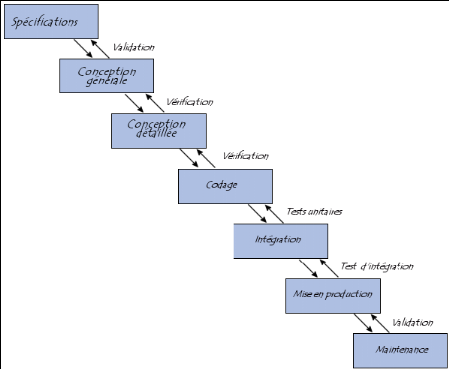
\includegraphics[width=0.60\textwidth,center]{img/cycle_en_cascade.png}


\subsection{modele en V}

Amélioration du modèle en cascade. Plier la ligne pour mettre en évidence la correspondance entre la production d’un produit et sa validation par des tests.\\
\\
\underline{Limites}: Inconvenient du modele en cascade.\\

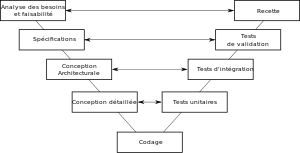
\includegraphics[width=0.60\textwidth,center]{img/cycle_en_v.png}


\subsection{modele en X}



\section{Modele non-lineaire}

Les détails de réalisation peuvent être reportés afin de produire une version opérationnelle du logiciel le plus tôt possible au cours du processus de développement.\\

\subsection{modele en Spirale}

Modèle cyclique convenant aux projets risqués.\\
Un cycle = un niveau du produit. Permet de fournir rapidement un prototype.\\
Le prototype se raffine progressivement jusqu'à l'obtention de l'application finale. Chaque cycle s'appuie sur les cycles précédents.\\ 

%%%%%%%%%\includegraphics{}

\underline{Limites} : Peut être fastidieux pour le client. Nécessite un cycle de développement rapide.\\
Peut amener à vouloir ajouter sans arrêt de nouvelles fonctionnalités. Ne s'applique pas à tous les types de projets.\\


\subsection{modele incrementale}

Le projet est découpé en sous-projet et chaque sous-projet est développé suivant un cycle en cascade(séquentiellement ou en parallèle)\\Un sous-projet = une ou plusieurs "grosses" fonctionnalités.\\
Chaque phase d’un sous-projet vient compléter la même phase d’un sous-projet.\\

\underline{Limite}: Dans certains cas, il peut être difficile de découper le projet en sous-projet du fait de fonctionnalités trop interdépendantes.\\
Chaque extension ne doit pas déstabiliser le logiciel déjà réalisé. Gestion du projet plus complexe (choix, planification et suivi des incréments).\\

%%%%%%%%%\includegraphics{}


\subsection{modele en fontaine}


%%%%%%%%%%%%%%%%%%%%%%%%%%%%%%%%%%%%%%%%%%%%%%

\newpage

\chapter{Diag. Gantt}
Le diagramme de Gantt permet de planifier et d'organiser des taches selon leur degrés d'importance et de leurs durée on peux donc voir l'avancement de chaque taches au cours d'un projets .
\\
\underline{Exemple de gantt} :\\
\\
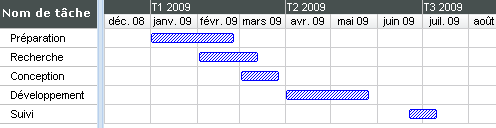
\includegraphics[width=0.60\textwidth,center]{img/gantt-diag.png}


%%%%%%%%%%%%%%%%%%%%%%%%%%%%%%%%%%%%%%%%%%%%%%%%%%%%%%%%%%%%%%%%%%%%%%%%%%%%%%%%%%%%%%%%%%%%
\newpage

\chapter{Diag. Pert}

Il s'agit d'un outil visuel d'ordonnancement et de planification de projet.\\
Son but est d'organiser les tâches sous la forme d'un réseau afin de faciliter la gestion du projet. Cette représentation graphique permet d'identifier les connexions entre les différentes tâches, les temps d'exécution, les interdépendances.\\
\\
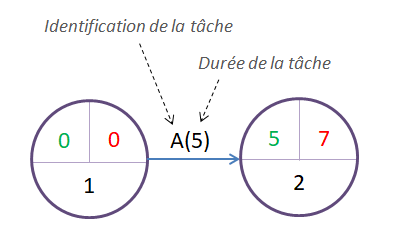
\includegraphics[width=0.60\textwidth,center]{img/pert-diag.png}

On remplie le cas du \textbf{plus tot} en premier en allant du debut a la fin en additionnant les duree des taches .Si une taches est précéde par 2 autres taches on choisi celle qui a la duree la plus longue pour additionné.\\
\\
On remplie la cas du \textbf{plus tard} en partant de la fin au debut en soustrayant les chemins des taches précédante . Si une taches est précéde par 2 autres taches on choisi celle qui a la duree la plus longue pour soustraire.\\

%%%%%%%%%%%%%%%%%%%%%%%%%%%%%%%%%%%%%%%%%%%%%%%%%%%%%%%%%%%%%%%%%%%%%%%%%%%%%%%%%%%%%%%%%%%%
\newpage

\chapter{SysML \& Scrum \& Merise \& Agile}

\section{SysMl}
Le passage de UML à SysML est très simple. Vous allez constater que les diagrammes sont moins nombreux et que SysML ré-utilise une bonne partie des diagrammes que vous connaissez déjà en UML (cf La Doc).\\
SysML est à l'ingénierie des systèmes complexes et/ou hétérogènes ce qu'UML est à l'informatique. SysML doit permettre à des acteurs de corps de métiers différents de collaborer autour d'un modèle commun pour définir un système.\\

%%%%%%%%%%%%%%%%%%%%%%%%%%%%%%%%%%%%%%%%%%%%%%%%%%%%%%%%%%%%%%%%%%%%%%%%%%%%%%%%%%%%%%%%%%%%
\newpage

\chapter{Diagramme UML}

\section{Diagramme des cas d'utilisation}

Comme son nom l'indique il s'agit d'un diagramme representer les acteur et interaction/fonctionnalité possible avec le systeme.\\
Le(s) acteur(s) princiaple est situé a gauche du schema et les acteurs secondaire sont placé a droite.\\
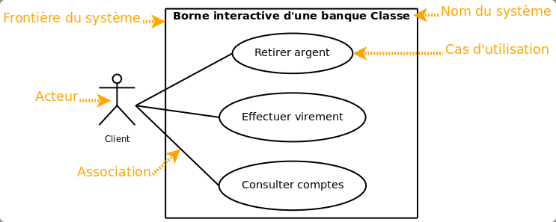
\includegraphics[width=0.60\textwidth,center]{img/diag_use_case.png}


\subsection{Relation d'inclusion et d'extension}

\underline{include}:\\
\\
Un cas A inclut un cas B si le comportement décrit par le cas A inclut le comportement du cas B : le cas A dépend de B. Lorsque A est sollicité, B l'est obligatoirement, comme une partie de A. Cette dépendance est symbolisée par le stéréotype \verb+<< include >>+.\\
La fleche est representer en pointillé et est noté du lavbel \verb+<<include>>+ (pareil pour \verb+<<extend>>+).\\

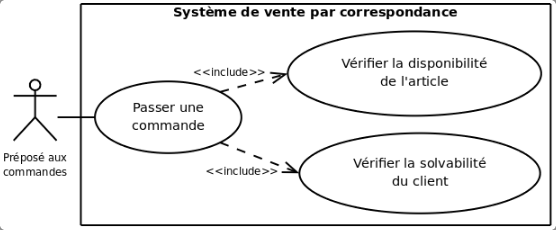
\includegraphics[width=0.60\textwidth,center]{img/include_relation.png}
\\

\underline{extend}:\\
\\
La relation d'extension est probablement la plus utile, car elle a une sémantique qui a un sens du point de vue métier au contraire des deux autres qui sont plus des artifices d'informaticiens.\\
On dit qu'un cas d'utilisation A étend un cas d'utilisation B lorsque le cas d'utilisation A peut être appelé au cours de l'exécution du cas d'utilisation B.\\
Exécuter B peut éventuellement entraîner l'exécution de A: contrairement à l'inclusion, l'extension est optionnelle. Cette dépendance est symbolisée par le stéréotype \verb+<< extend >>+.\\


\section{diagramme de classe}

\subsection{Vocabulaire}

Une \textbf{instance} est une concrétisation d'un concept abstrait. \\
\\
\underline{Exemple}:\\
-La Ferrari Enzo qui se trouve dans votre garage est une instance du concept abstrait Automobile;\\
-L'amitié qui lie Jean et Marie est une instance du concept abstrait Amitié;\\
\\
\\
Une \textbf{classe} est un concept abstrait représentant des éléments variés comme:\\
\\
-des éléments concrets (ex. : des avions)\\
-des éléments abstraits (ex. : des commandes de marchandises ou services)\\
-des composants d'une application (ex. : les boutons des boîtes de dialogue)\\
-des structures informatiques (ex. : des tables de hachage)\\
-des éléments comportementaux (ex. : des tâches), etc.\\
\\
Tout système orienté objet est organisé autour des classes.\\
Une classe est la description formelle d'un ensemble d'objets ayant une sémantique et des caractéristiques communes.\\
\\
Un \textbf{objet} est une instance d'une classe. C'est une entité discrète dotée d'une identité, d'un état et d'un comportement que l'on peut invoquer. Les objets sont des éléments individuels d'un système en cours d'exécution.\\


\subsection{Encapsulation et visibilité}

L'encapsulation est un mécanisme consistant à rassembler les données et les méthodes au sein d'une structure en cachant l'implémentation de l'objet, c'est-à-dire en empêchant l'accès aux données par un autre moyen que les services proposés.\\
Ces services accessibles (offerts) aux utilisateurs de l'objet définissent ce que l'on appelle l'interface de l'objet (sa vue externe).\\
\\
L'encapsulation permet donc de garantir l'intégrité des données contenues dans l'objet.L'encapsulation permet de définir des niveaux de visibilité des éléments d'un conteneur.\\
\\
-\textbf{Public ou + }:\\
tout élément qui peut voir le conteneur peut également voir l'élément indiqué.\\
\\
-\textbf{Protected ou \# }:\\
seul un élément situé dans le conteneur ou un de ses descendants peut voir l'élément indiqué.\\
\\
-\textbf{Private ou - }:\\
seul un élément situé dans le conteneur peut voir l'élément.\\
\\
-\textbf{Package ou \∼ ou rien} :\\
seul un élément déclaré dans le même paquetage peut voir l'élément.\\
\\

\subsection{Relation association}

Permet de faire la liaison entre 2 classe.\\
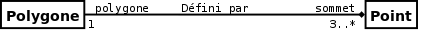
\includegraphics[width=0.60\textwidth,center]{img/relation_association.png}


\subsection{Relation heritage}

La relation d'heritage permet de dire aux classe parent qu'il ont acces aux attributs des classe enfant.
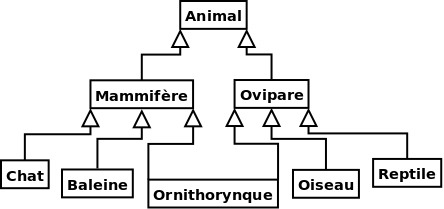
\includegraphics[width=0.60\textwidth,center]{img/relation_heritage.png}
\\
On peux marqu\'e sous le relation \verb+{overlapping}+ quand 2 roles d'une classe peuvent d'inverser par exemple etudiant et enseignant (un etudiant peux enseigner).

\subsection{Relation agregation et composition}

La flèche en forme de losange , celle en blanche designe l'agregation . Cela signifie qu'un partie du systeme est composé de ... Si celui ci venait a disparaitre le reste du systeme lui continuera d'exister.\\
\\
La flèche en forme de losange noir lui signifie la composition , si on supprime une partie du systeme c'est tout le systeme qui cesse d'exister.\\
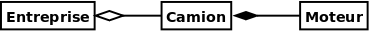
\includegraphics[width=0.60\textwidth,center]{img/relation_agregat_et_composition.png}


\end{document}
